\documentclass{beamer}
% Use DS9 global theme (includes pgfplots for visualization)
\usepackage{../../../shared/templates/ds9_theme}

% Title page configuration
\title[Switch and While Loops]{CS12 CH: Switch Statements and While Loops}
\subtitle{Control Structures and Iteration}
\author[Mr. Gullo]{Mr. Gullo}
\date[Oct 2025]{October 2025}

\begin{document}
\frame{\titlepage}

\section{Control Structures}

\begin{frame}
\frametitle{Learning Objectives}
By the end of this lesson, you will be able to:
\begin{itemize}
\item Compare switch statements with if/else chains and identify appropriate use cases
\pause
\item Implement while loops with proper initialization, condition testing, and updates
\pause
\item Distinguish between pre-increment (++x) and post-increment (x++) operators and predict their behavior in expressions
\pause
\item Identify and debug infinite loops in code
\pause
\item Apply while loops to solve mathematical problems involving sequences and series
\end{itemize}
\end{frame}

\begin{frame}
\frametitle{Switch Statements: Overview}
A \textbf{switch statement} is a control structure that executes different code blocks based on the value of a single variable or expression.

\textbf{Key Components:}
\begin{itemize}
\item \texttt{switch(expression)} - evaluates once
\pause
\item \texttt{case label:} - matches specific values
\pause
\item \texttt{break;} - exits the switch
\pause
\item \texttt{default:} - catches unmatched values (optional)
\end{itemize}

\textbf{Advantages:}
\begin{itemize}
\item More readable for multiple equality comparisons
\pause
\item Compact structure compared to long if/else chains
\pause
\item Clear handling of multiple options
\end{itemize}
\end{frame}

\begin{frame}
\frametitle{When to Use Switch vs If/Else}
Understanding when to use each control structure is important for writing clear, efficient code.

\textbf{Use Switch When:}
\begin{itemize}
\item Testing equality with multiple constant values
\pause
\item Working with integers, characters, or enums
\pause
\item Code readability benefits from case organization
\end{itemize}

\pause
\textbf{Use If/Else When:}
\begin{itemize}
\item Testing ranges or complex conditions
\pause
\item Using logical operators (AND, OR, NOT)
\pause
\item Comparing floating point numbers
\pause
\item Need inequality comparisons ($<$, $>$, $\leq$, $\geq$)
\end{itemize}
\end{frame}

\begin{frame}[fragile]
\frametitle{Switch vs If/Else: Side-by-Side Comparison}
Both accomplish the same goal but switch is more compact for multiple equality checks.

\pause
\begin{columns}[t]
\column{0.48\textwidth}
\textbf{If/Else Chain:}
\begin{minted}[fontsize=\tiny]{cpp}
if(option == 'A')
    cout << "Excellent!" << endl;
else if(option == 'B' || option == 'C')
    cout << "Well done" << endl;
else if(option == 'D')
    cout << "You passed" << endl;
else if(option == 'F')
    cout << "Better try again" << endl;
else
    cout << "Invalid grade" << endl;
\end{minted}

\column{0.48\textwidth}
\textbf{Switch Statement:}
\begin{minted}[fontsize=\tiny]{cpp}
switch(option) {
    case 'A':
        cout << "Excellent!" << endl;
        break;
    case 'B':
    case 'C':
        cout << "Well done" << endl;
        break;
    case 'D':
        cout << "You passed" << endl;
        break;
    case 'F':
        cout << "Better try again" << endl;
        break;
    default:
        cout << "Invalid grade" << endl;
}
\end{minted}
\end{columns}
\end{frame}

\begin{frame}
\frametitle{Important Switch Features}
\textbf{Break Statement:}
\begin{itemize}
\item Terminates switch execution
\pause
\item Transfers control to statement after switch
\pause
\item Without break, execution "falls through" to next case
\end{itemize}

\pause
\textbf{Fall-Through Behavior:}
\begin{itemize}
\item Multiple cases can share the same code block
\pause
\item Example: \texttt{case 'B':} and \texttt{case 'C':} both execute same code
\pause
\item Intentional fall-through can be useful but requires care
\end{itemize}

\pause
\textbf{Default Case:}
\begin{itemize}
\item Executes when no other case matches
\pause
\item Optional but recommended for robust code
\pause
\item Handles unexpected input gracefully
\end{itemize}
\end{frame}

\section{While Loops}

\begin{frame}
\frametitle{While Loops: Fundamentals}
A \textbf{while loop} repeatedly executes a block of code as long as a condition remains true.

\textbf{Structure:}
\begin{enumerate}
\item \textbf{Initialization} - setup before loop
\pause
\item \textbf{Condition} - tested before each iteration
\pause
\item \textbf{Loop body} - code to execute
\pause
\item \textbf{Update} - modify variables to eventually exit loop
\end{enumerate}

\textbf{Key Characteristics:}
\begin{itemize}
\item Pre-test loop: condition checked before body executes
\pause
\item May execute zero times if condition initially false
\pause
\item Must have proper update to avoid infinite loops
\end{itemize}
\end{frame}

\begin{frame}
\frametitle{While Loop Execution Flow}
Understanding the order of operations in a while loop is crucial for predicting program behavior. The loop follows a specific sequence from initialization through termination.

\pause
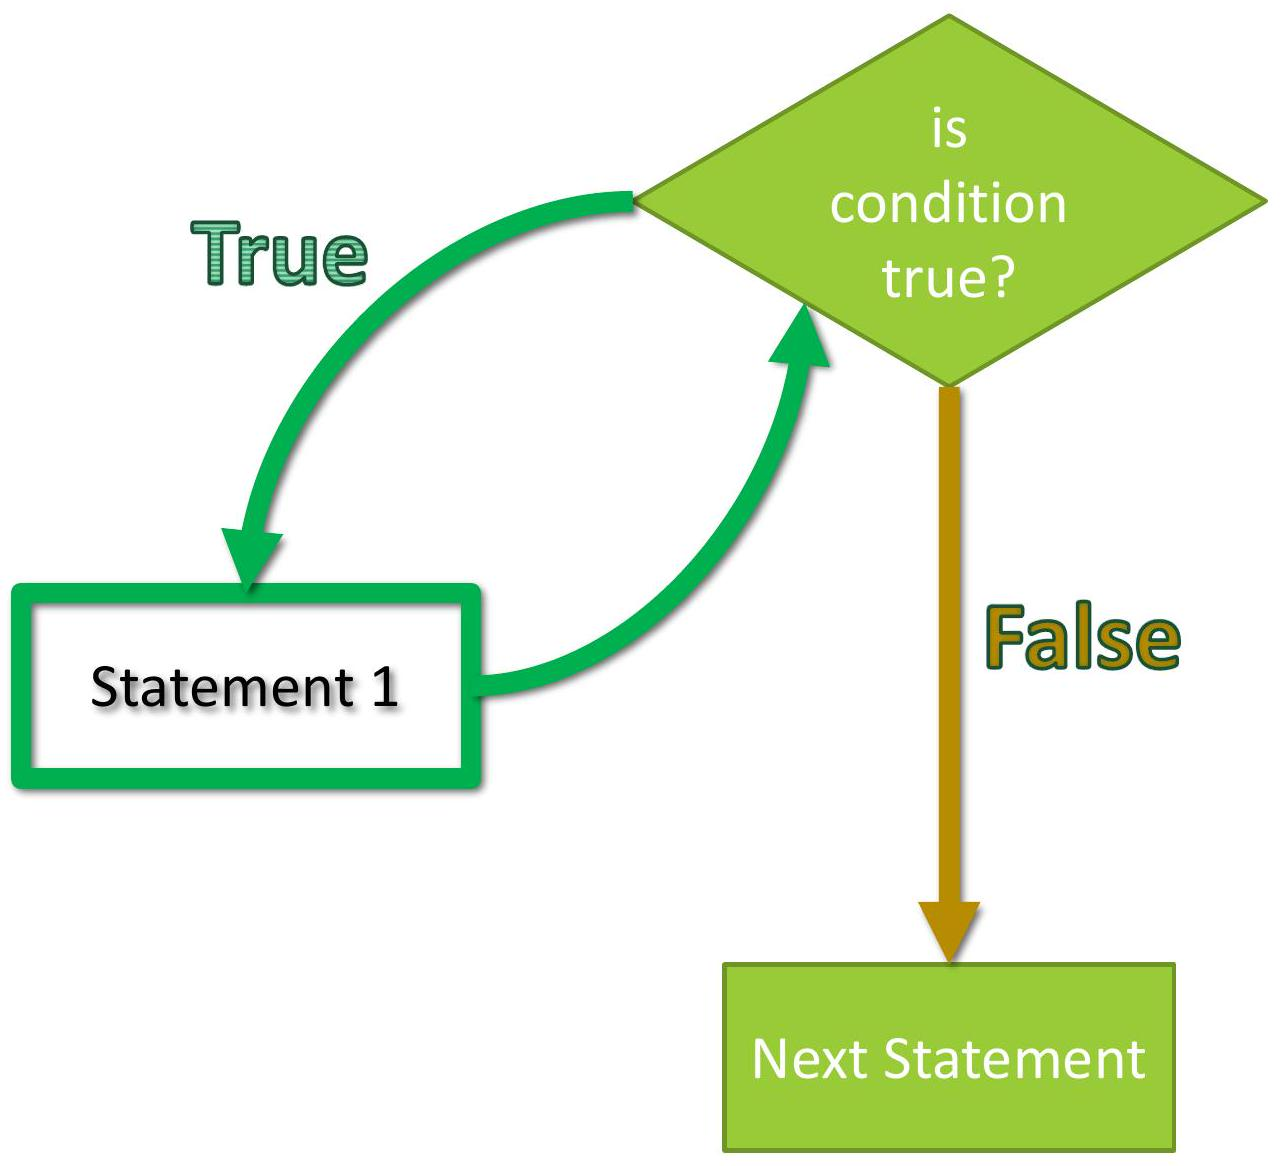
\includegraphics[width=0.6\textwidth]{../images/While-Loop-Flowchart.jpg}
\end{frame}

\begin{frame}[fragile]
\frametitle{Basic While Loop Example}
\textbf{Reference File:} \texttt{02\_whileLoopsIntro.cpp}

\pause
\begin{minted}[fontsize=\small]{cpp}
#include <iostream>
using namespace std;

int main() {
    int countDown = 10;
    while(countDown >= 0) {
        cout << countDown << '\n';
        countDown = countDown - 1;
    }
    return 0;
}
\end{minted}

\pause
\textbf{Output:} 10 9 8 7 6 5 4 3 2 1 0

The loop executes 11 times, printing values from 10 down to 0.
\end{frame}

\section{Operators}

\begin{frame}
\frametitle{Increment and Decrement Operators}
C++ provides shorthand operators for increasing or decreasing a variable by one.

\textbf{Post-Increment/Decrement (x++, x--):}
\begin{itemize}
\item Uses current value in expression
\pause
\item Then increments/decrements the variable
\pause
\item Example: if x=5, then y=x++ results in y=5, x=6
\end{itemize}

\textbf{Pre-Increment/Decrement (++x, --x):}
\begin{itemize}
\item Increments/decrements the variable first
\pause
\item Then uses new value in expression
\pause
\item Example: if x=5, then y=++x results in y=6, x=6
\end{itemize}
\end{frame}




\begin{frame}
\frametitle{Pre vs Post: Understanding the Difference}
The timing of when the increment or decrement occurs relative to when the value is used makes a critical difference in loop behavior and expressions. This affects both the values displayed and the number of iterations.
\end{frame}

\begin{frame}[fragile]
\frametitle{Pre vs Post: Execution Trace}
\pause
\begin{columns}[t]
\column{0.48\textwidth}
\textbf{Post-Decrement:}
\begin{minted}[fontsize=\tiny]{cpp}
int countDown = 10;
while(countDown-- >= 0) {
    cout << countDown << '\n';
}
\end{minted}
\pause
\textbf{Trace:}
\begin{itemize}
\item Test: 10 $\geq$ 0? Yes
\item Print: 9 (after decrement)
\item Test: 9 $\geq$ 0? Yes
\item Print: 8
\item ... continues to -1
\end{itemize}
\textbf{Output:} 9 8 7 6 5 4 3 2 1 0 -1

\column{0.48\textwidth}
\textbf{Pre-Decrement:}
\begin{minted}[fontsize=\tiny]{cpp}
int countDown = 10;
while(--countDown >= 0) {
    cout << countDown << '\n';
}
\end{minted}
\pause
\textbf{Trace:}
\begin{itemize}
\item Decrement to 9, test: 9 $\geq$ 0? Yes
\item Print: 9
\item Decrement to 8, test: 8 $\geq$ 0? Yes
\item Print: 8
\item ... continues to 0
\end{itemize}
\textbf{Output:} 9 8 7 6 5 4 3 2 1 0
\end{columns}
\end{frame}

\begin{frame}
\frametitle{Infinite Loops}
An \textbf{infinite loop} is a loop that continues indefinitely because its termination condition is never met.

\textbf{Common Causes:}
\begin{itemize}
\item Missing update statement
\pause
\item Incorrect condition logic
\pause
\item Update moves away from termination condition
\end{itemize}

\textbf{Example of Infinite Loop:}
\begin{itemize}
\item \texttt{int x = 1;}
\item \texttt{while(x < 500)}
\item \texttt{cout << x << endl;}
\end{itemize}

Problem: x never changes, so condition always true. Solution: add \texttt{x++;} inside loop.
\end{frame}

\section{Applications and Exercises}

\begin{frame}
\frametitle{Essential Formulas: Arithmetic Sequences}
\textbf{Arithmetic Sequence:} Each term differs from previous by constant difference d.

\pause
\textbf{nth Term Formula:}
$$a_n = t + (n-1)d$$
where t = first term, d = common difference, n = term number

\pause
\textbf{Series Sum Formula (first n terms):}
$$S_n = \frac{n(t + a_n)}{2}$$
where $a_n$ is the nth term

\pause
\textbf{Example:} Sequence 2, 5, 8, 11, ... has t=2, d=3
\begin{itemize}
\item 5th term: $a_5 = 2 + (5-1)(3) = 14$
\pause
\item Sum of first 5 terms: $S_5 = \frac{5(2+14)}{2} = 40$
\end{itemize}
\end{frame}

\begin{frame}
\frametitle{Essential Formulas: Geometric Sequences}
\textbf{Geometric Sequence:} Each term is previous term multiplied by constant ratio r.

\pause
\textbf{nth Term Formula:}
$$a_n = t \cdot r^{n-1}$$
where t = first term, r = common ratio, n = term number

\pause
\textbf{Series Sum Formula (first n terms):}
$$S_n = \frac{t(1-r^n)}{1-r} \text{ when } r \neq 1$$

\pause
\textbf{Example:} Sequence 3, 6, 12, 24, ... has t=3, r=2
\begin{itemize}
\item 5th term: $a_5 = 3 \cdot 2^{5-1} = 48$
\pause
\item Sum of first 5 terms: $S_5 = \frac{3(1-2^5)}{1-2} = 93$
\end{itemize}
\end{frame}

\begin{frame}[fragile]
\frametitle{Demo: Triangle Numbers}
\textbf{Demo File:} \texttt{03\_triangleNumbers.cpp}

\pause
Triangle numbers are cumulative sums: 1, 3, 6, 10, 15, ...

\pause
\begin{minted}[fontsize=\tiny]{cpp}
#include <iostream>
using namespace std;

int main() {
    int n;
    int sum = 0;
    int current_n = 1;
    
    cout << "Please enter an integer: ";
    cin >> n;
    
    cout << "The first " << n << " triangle numbers are:\n";
    
    while(current_n <= n) {
        sum = sum + current_n;
        cout << "Term Number: " << current_n;
        cout << "\tSum: " << sum;
        cout << "\tFormula: " << current_n*(current_n+1)/2 << endl;
        current_n++;
    }
    return 0;
}
\end{minted}
\end{frame}

\begin{frame}
\frametitle{Leap Year Logic}
A year is a leap year if it meets specific divisibility criteria.

\pause
\textbf{Leap Year Rules:}
\begin{itemize}
\item Divisible by 400: Always a leap year
\pause
\item Divisible by 100 (but not 400): Not a leap year
\pause
\item Divisible by 4 (but not 100): Leap year
\pause
\item Otherwise: Not a leap year
\end{itemize}

\pause
\textbf{Boolean Expression:}
$$(year \% 400 == 0) \text{ OR } (year \% 4 == 0 \text{ AND } year \% 100 \neq 0)$$

\pause
\textbf{Examples:}
\begin{itemize}
\item 2000: Leap (divisible by 400)
\pause
\item 1900: Not leap (divisible by 100 but not 400)
\pause
\item 2024: Leap (divisible by 4 but not 100)
\end{itemize}
\end{frame}

\begin{frame}[fragile]
\frametitle{Exercise 1: Switch Statement Practice}
\textbf{Exercise File:} \texttt{01elseIf\_vs\_switch.cpp} (Template with TODOs)

\pause
\textbf{Objective:} Convert an if/else chain to a switch statement.

\begin{minted}[fontsize=\scriptsize]{cpp}
#include <iostream>
using namespace std;

int main() {
    char option;
    cout << "Enter grade (A/B/C/D/F): ";
    cin >> option;
    
    // TODO 1: Create switch statement for option variable
    // TODO 2: Add case for 'A' that prints "Excellent!"
    // TODO 3: Add cases for 'B' and 'C' (same output: "Well done")
    // TODO 4: Add case for 'D' that prints "You passed"
    // TODO 5: Add case for 'F' that prints "Better try again"
    // TODO 6: Add default case for invalid input
    // TODO 7: Remember to add break statements after each case
    
    return 0;
}
\end{minted}
\end{frame}

\begin{frame}[fragile]
\frametitle{Exercise 2: While Loop Countdown}
\textbf{Exercise File:} \texttt{02\_whileLoopsIntro.cpp} (Template with TODOs)

\pause
\textbf{Objective:} Practice while loops and observe pre/post decrement differences.

\begin{minted}[fontsize=\scriptsize]{cpp}
#include <iostream>
using namespace std;

int main() {
    int countDown = 10;
    
    // TODO 1: Create while loop that continues while countDown >= 0
    // TODO 2: Inside loop, print the current value of countDown
    // TODO 3: Decrement countDown using: countDown = countDown - 1
    // TODO 4: After testing, try replacing decrement with countDown--
    // TODO 5: Try again with --countDown and compare outputs
    // TODO 6: Document which version (post or pre) prints 10 to 0
    
    return 0;
}
\end{minted}

\textbf{Expected outputs:} Original prints 10-0. Post-decrement in condition changes behavior.
\end{frame}

\begin{frame}[fragile]
\frametitle{Exercise 3: Leap Years}
\textbf{Exercise File:} \texttt{ex1\_leapYears.cpp} (Template with TODOs)

\pause
\textbf{Objective:} Display leap years in a given range using a while loop.

\begin{minted}[fontsize=\tiny]{cpp}
#include <iostream>
using namespace std;

int main() {
    int yearFrom, yearTo;
    
    cout << "Please enter the starting year: ";
    cin >> yearFrom;
    cout << "Please enter the ending year: ";
    cin >> yearTo;
    
    // TODO 1: Validate that yearFrom <= yearTo (exit if not)
    
    cout << "The leap years between " << yearFrom 
         << " and " << yearTo << " are:\n";
    
    // TODO 2: Create while loop from yearFrom to yearTo (inclusive)
    // TODO 3: Inside loop, test if current year is leap year using formula
    // TODO 4: Formula: (year % 400 == 0) OR (year % 4 == 0 AND year % 100 != 0)
    // TODO 5: If leap year, print it
    // TODO 6: Increment year counter
    
    return 0;
}
\end{minted}
\end{frame}

\begin{frame}[fragile]
\frametitle{Exercise 4: Arithmetic Sequences Using Formulas}
\textbf{Exercise File:} \texttt{ex2\_arithmeticFormulas.cpp} (Template with TODOs)

\pause
\textbf{Objective:} Generate arithmetic sequence and series using formulas.

\begin{minted}[fontsize=\tiny]{cpp}
#include <iostream>
using namespace std;

int main() {
    int t, n, d;
    int termNumber = 1;
    
    cout << "Please enter the starting term: ";
    cin >> t;
    cout << "Please enter the common difference: ";
    cin >> d;
    cout << "Please enter the number of terms: ";
    cin >> n;
    
    cout << "Term\tSequence\tSeries\n";
    
    // TODO 1: Create while loop from termNumber 1 to n
    // TODO 2: Calculate current term using formula: t + (termNumber-1)*d
    // TODO 3: Calculate series sum using formula: termNumber*(t+currentTerm)/2
    // TODO 4: Print: termNumber, currentTerm, and series sum
    // TODO 5: Increment termNumber
    
    return 0;
}
\end{minted}
\end{frame}

\begin{frame}[fragile]
\frametitle{Exercise 5: Geometric Sequences Without Formulas}
\textbf{Exercise File:} \texttt{ex3\_geometricCumulative.cpp} (Template with TODOs)

\pause
\textbf{Objective:} Build geometric sequence and series using repeated multiplication/addition.

\begin{minted}[fontsize=\tiny]{cpp}
#include <iostream>
using namespace std;

int main() {
    int t, n, r;
    int termNumber = 1;
    int currentSum = 0;
    int currentTerm = t;
    
    // TODO 1: Prompt user for t (first term), r (ratio), n (number of terms)
    
    cout << "Term\tSequence\tSeries\n";
    
    // TODO 2: Create while loop from termNumber 1 to n
    // TODO 3: Add currentTerm to currentSum (building series)
    // TODO 4: Print: termNumber, currentTerm, and currentSum
    // TODO 5: Calculate next term by multiplying currentTerm by r
    // TODO 6: Increment termNumber
    
    return 0;
}
\end{minted}

\textbf{Note:} Use multiplication for next term, not the formula $t \cdot r^{n-1}$.
\end{frame}

\begin{frame}[fragile]
\frametitle{Exercise 6: Triangle Numbers}
\textbf{Exercise File:} \texttt{while-loops-example.cpp} (Template with TODOs)

\pause
\textbf{Objective:} Calculate triangle numbers using both cumulative sum and formula.

\begin{minted}[fontsize=\tiny]{cpp}
#include <iostream>
using namespace std;

int main() {
    int n;
    int sum = 0;
    int current_n = 1;
    
    cout << "Please enter an integer: ";
    cin >> n;
    
    cout << "The first " << n << " triangle numbers are:\n";
    
    // TODO 1: Create while loop from current_n to n (inclusive)
    // TODO 2: Add current_n to sum (cumulative approach)
    // TODO 3: Print term number (current_n)
    // TODO 4: Print cumulative sum
    // TODO 5: Calculate using formula: current_n*(current_n+1)/2
    // TODO 6: Print formula result (should match sum)
    // TODO 7: Increment current_n
    
    return 0;
}
\end{minted}
\end{frame}

\begin{frame}
\frametitle{Summary}
\textbf{Key Takeaways:}
\begin{itemize}
\item Switch statements provide compact, readable code for multiple equality comparisons but are limited to discrete values
\pause
\item While loops require careful attention to initialization, condition testing, and updates to avoid infinite loops
\pause
\item Pre-increment (++x) and post-increment (x++) differ in when the value changes relative to when it is used in expressions
\pause
\item Mathematical sequences can be implemented using either formulas (arithmetic) or iterative accumulation (geometric)
\pause
\item Proper loop structure with clear termination conditions is essential for reliable programs
\end{itemize}

\pause
\textbf{Practice:} Complete all six exercises to master these concepts.
\end{frame}

\end{document}